A fundamentação teórica para a elaboração deste trabalho consiste em conceitos ligados ao \emph{Machine Learning}. Primeiramente, os conceitos gerais desta área serão apresentados na Seção \ref{subsec:ml}, seguidos pelas características das Redes Neurais Artificais na Seção \ref{subsec:rna}. As definições elementares da técnica de \emph{Machine Learning} conhecida como \emph{Deep Learning} são apresentadas na Seção \ref{subsec:dl}. A Seção \ref{subsubsec:cnns} discorre sobre as características das Redes Neurais Convolucionais, prosseguindo até a Seção \ref{subsubsec:arq-cnns} onde são apresentadas algumas de suas arquiteturas canônicas. Por fim, a Seção \ref{subsubsec:transfer} contém informações sobre a técnica conhecida como \emph{Transfer Learning}, um conceito emergente utilizado em aplicações de \emph{Deep Learning}.

%%%%%

\subsection{\emph{Machine Learning}}
\label{subsec:ml}

\emph{Machine Learning} (ML), também conhecido como Aprendizado de Máquina, é o estudo sistemático de algoritmos e sistemas que melhoram seu conhecimento ou desempenho com o uso da experiência \cite{flach}. Em 1959, o pioneiro em jogos de computador Arthur Samuels definiu \emph{Machine Learning} como um ``campo de estudos que dá aos computadores a habilidade de aprender sem serem explicitamente programados'' \cite{simon}. De acordo com Murphy \cite{murphy} , \emph{Machine Learning} pode ser definido como um conjunto de métodos que podem detectar padrões em dados automaticamente e, em seguida, utilizar os padrões detectados para predizer dados futuros, ou para realizar outros tipos de decisão sob algum tipo de incerteza.

O \emph{Machine Learning} é comumente dividido em três tipos principais de aprendizado, chamados de supervisionado, não-supervisionado e semi-supervisionado. No caso dos algoritmos de aprendizado supervisionado, o objetivo é aprender um mapeamento de entradas para saídas, dado um conjunto rotulado de pares de entradas e saídas. No aprendizado não supervisionado, o algoritmo é apresentado somente aos dados de entrada, e o seu propósito é encontrar padrões significativos nos mesmos. Este problema não é bem definido, porque geralmente não é especificado o tipo de padrão que deve ser encontrado nos dados. Além disso, diferentemente do aprendizado supervisionado, não existe nenhuma métrica de erro óbvia para utilizar. O aprendizado semi-supervisionado, por sua vez, normalmente combina uma pequena quantidade de dados rotulados com uma grande quantidade de dados não rotulados para criar um classificador próprio. Em alguns casos, a abordagem de aprendizagem semi-supervisionada pode ser de grande valor prático. \cite{khan}

Como mostrado na Figura \ref{fig:tasks}, utilizar os atributos corretos para construir os modelos certos que conquistam determinadas tarefas é a essência de ML. Atributos podem ser definidos como uma ``linguagem'' que descreve os objetos relevantes no domínio do problema. Tendo a representação característica adequada dos objetos do domínio, normalmente, não é necessário retornar ao objeto em si, e é por isso que os atributos têm um papel importante em ML. A tarefa é uma representação abstrata de um problema que deseja-se resolver levando em consideração os objetos do domínio. Dentre as tarefas de aprendizado supervisionado mais utilizadas estão a tarefa de classificação binária ou multiclasse e a tarefa de regressão. Um modelo, por sua vez, é a saída produzida por dados de treinamento aplicados em determinado algoritmo de ML \cite{flach}.

\begin{figure}
\centering
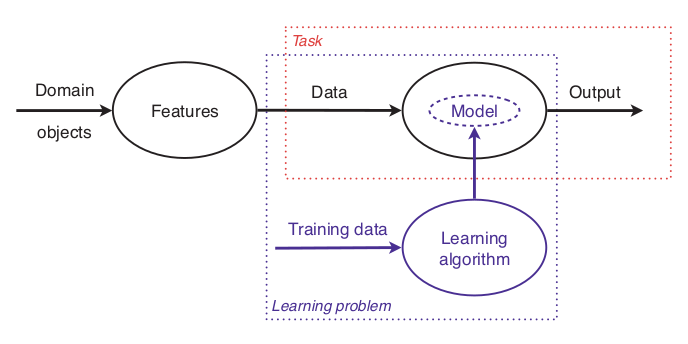
\includegraphics[height=5cm]{imgs/tasks}
\caption{Uma visão geral de como ML é utilizado para adereçar uma tarefa. Fonte: \cite{flach}.}
\label{fig:tasks}
\end{figure}


Em uma tarefa de classificação, um algoritmo é selecionado para especificar quais das $k$ categorias possíveis uma entrada pertence. Para resolver essa tarefa, o algoritmo de aprendizado normalmente produz uma função $f : I\!R^n \rightarrow {1,...,k}$. Quando $y = f(x)$, o modelo denomina uma entrada descrita com o vetor $x$ para uma categoria identificado por um valor numérico $y$ \cite{goodfellow}. Alguns exemplos de tarefa de classificação são a detecção de faces em imagens, a determinação do gênero do indíviduo nessas imagens, a verificação da espécie de uma planta, entre outros.

Quanto à tarefa de regressão, é solicitado a um programa a predição de um valor numérico a partir de uma entrada. Desta forma, o algoritmo de aprendizado é proposto a retornar uma função $f : I\!R^n \rightarrow I\!R$ \cite{goodfellow}. Algumas tarefas de regressão podem ser, por exemplo, a determinação do valor de uma corrida de táxi, a identificação da idade de um indivíduo em uma imagem, prever o preço de uma casa baseado nos dados de casas vendidas anteriormente, etc.

Dentre os tipos de modelos existentes, podemos citar os geométricos, probabilísticos e lógicos. Um modelo geométrico é construído diretamente em função do espaço, utilizando-se de conceitos geométricos como linhas, planos e distâncias. Como exemplos de modelos geométricos temos a regressão linear, o \emph{perceptron} e, em consequência, as redes neurais artificiais. Nos modelos probabilísticos, como o classificador Bayesiano, a questão principal é modelar a relação entre os dados de entrada e saída assumindo que existe algum processo aleatório implícito que produz os valores para essas variáveis, de acordo com uma distribuição de probabilidade bem definida, porém desconhecida. Um modelo lógico, em contrapartida, é o mais naturalmente algorítmico, considerando a capacidade de ser facilmente transformado em regras que podem ser entendidas por seres humanos. Dentre os modelos lógicos estão as árvores de decisão, onde as suas folhas são rotuladas para caracterizar o tipo de tarefa associado ao modelo \cite{flach}.

Dentre os modelos geométricos, as redes neurais artificiais têm demonstrado grande desempenho em diversas áreas. Aplicações de \emph{Deep Learning} para detecção de padrões em imagens e reconhecimento de voz, por exemplo, utilizam-se desses modelos para a obtenção de resultados relevantes. Tomando isto e levando em consideração o contexto deste trabalho, as próximas seções apresentadas abordam significativamente estes conceitos.

%%%%%

\subsection{Redes Neurais Artificiais}
\label{subsec:rna}

As \emph{Redes Neurais Artificiais} (RNAs) são uma tentativa computacional de modelar a capacidade de processamento de informação do sistema nervoso humano \cite{rojas}. Para alcançarem um bom desempenho, as RNAs empregam uma interligação de estruturas bases chamadas de neurônios artificiais que, por sua vez, possuem pesos com valores numéricos positivos ou negativos associados a si. Uma vantagem das RNAS, é a grande capacidade de generalização, ou seja, a habilidade de produzir saídas adequadas para entradas que não estavam presente anteriormente durante sua aprendizagem \cite{haykin}. As RNAs têm sido frequentemente utilizadas nas áreas de processamento de sinais, reconhecimento de padrões, medicina, reconhecimento de voz, negócios, entre outras \cite{fausett}.

A idealização dos neurônios artificiais foi inspirada nos neurônios biológicos encontrados no cérebro humano. Como mostrado na Figura \ref{fig:sinapse}, cada neurônio biológico é composto pelo corpo celular, os dendritos e o axônio. Os dendritos têm como papel a recepção das informações, ou impulsos nervosos, de outros neurônios e submetê-las ao corpo celular, onde as informações são processadas e novos impulsos são gerados. Estes impulsos são enviados aos dendritos de outros neurônios através do axônio. O ponto de contato entre os neurônios através do axônio e os dentritos, denominado sinapse, é onde ocorre toda a troca de informação necessária para conceber uma rede neural \cite{braga}.

\begin{figure}
\centering
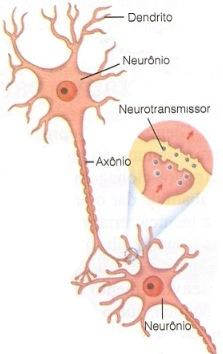
\includegraphics[height=5cm]{imgs/sinapse}
\caption{Estrutura de um neurônio e zona de conexão funcional entre as células (sinapse) \cite{sinapse}.}
\label{fig:sinapse}
\end{figure}


Um neurônio biológico dispara quando a soma dos impulsos que ele recebe ultrapassa o seu limiar de excitação, denominado \emph{threshold}. O corpo do neurônio é controlado por um mecanismo simples que faz a soma dos valores $x_i w_i$ recebidos pelos seus dendritos e decide se o neurônio deve ou não disparar, comparando a soma obtida com o \emph{threshold} do neurônio. No modelo de neurônio artificial proposto por McCulloch e Pitts (MCP) em \cite{mcculloch}, a ativação do neurônio é obtida através da aplicação de uma \emph{função de ativação}, que ativa ou não a saída, dependendo do valor da soma ponderada das suas entradas, como é mostrado na Figura \ref{fig:neuronio-artificial} \cite{braga}.

\begin{figure}[H]
\centering
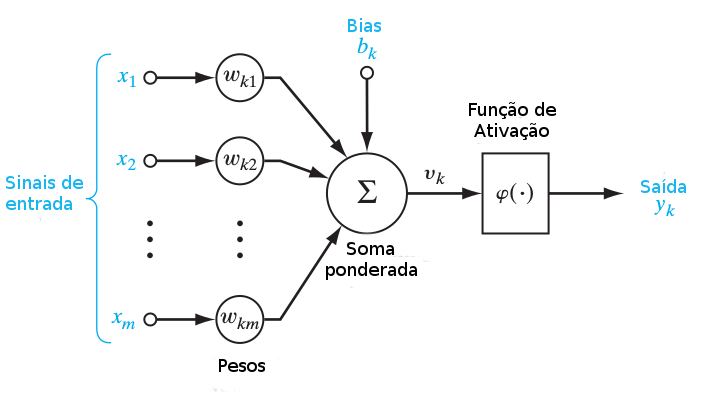
\includegraphics[height=6cm]{imgs/neuronio-artificial}
\caption{Estrutura de um neurônio artificial. Fonte: \cite{haykin}}
\label{fig:neuronio-artificial}
\end{figure}

Uma função de ativação $\varphi$ é responsável por determinar a saída $y$ do neurônio, a partir das entradas $x = x_1, ..., x_n$ e pesos $w = w_1, ..., w_n$. A maioria dos modelos de neurônio utiliza ainda um \emph{bias} externo aplicado, denotado na Figura \ref{fig:neuronio-artificial} como $b_k$. Este bias é utilizado para o aumentar ou diminuir os valores de entrada da função de ativação, dependendo se o seu valor é positivo ou negativo, respectivamente \cite{haykin}. No caso do neurônio MCP, a funçao de ativação é do tipo degrau deslocada e é comparada ao seu \emph{threshold} $\theta$, como mostrado nas Equações \ref{eq:soma-ponderada} e \ref{eq:degrau}.

\begin{equation}
  \label{eq:soma-ponderada}
  v(x,w) = \sum\limits_{i=1}^n x_i w_i + b
\end{equation}

\begin{equation}
\label{eq:degrau}
\varphi(v) = \left\{
\begin{array}{lr}
  1, & \text{se } v > \theta\\
  0, & \text{caso contrário}
\end{array}
\right.
\end{equation}

Para a correta funcionalidade de determinados algoritmos em RNAs, como o de \emph{backpropagation} em redes \emph{multilayer perceptron}, sabe-se que a escolha da função de ativação deve considerar funções contínuas e diferenciáveis \cite{haykin}. As funções identidade, sigmóide, tangente hiperbólica e retificada linear (ReLU) são as mais utilizadas no processo de construção de RNAs. Algumas propriedades dessas funcões estão apresentadas na Figura \ref{fig:activation}.

\begin{figure}[h!]
     \subfloat[Identidade ou Linear\label{subfig:identity}]{%
       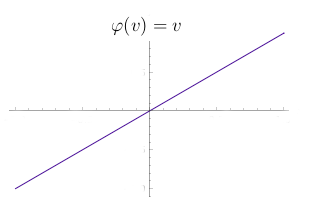
\includegraphics[width=0.4\textwidth]{imgs/identity}
     }
     \hfill
     \subfloat[Tangente Hiperbólica\label{subfig:tanh}]{%
       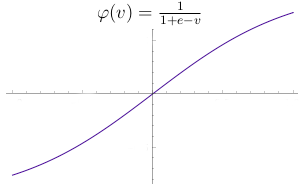
\includegraphics[width=0.4\textwidth]{imgs/tanh}
     }
     \hfill
     \subfloat[Sigmóide ou Logística\label{subfig:sigmoid}]{%
       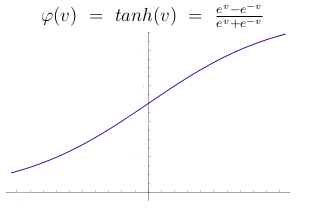
\includegraphics[width=0.4\textwidth]{imgs/sigmoid}
     }
     \hfill
     \subfloat[Unidade Linear Retificada (ReLu)\label{subfig:relu}]{%
       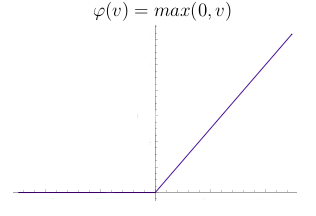
\includegraphics[width=0.4\textwidth]{imgs/relu}
     }
     \caption{Exemplos de funções de ativação \cite{goodfellow}}
     \label{fig:activation}
\end{figure}


Em 1958, visando a melhoria do neurônio MCP, Frank Rosenblatt desenvolveu o modelo \emph{Perceptron} \cite{Rosenblatt}. Neste modelo, criou-se o primeiro conceito de aprendizagem através de neurônios artificiais, onde foi projetada uma regra de correção de erros para modificar os pesos associados a um neurônio quando suas respostas aos estímulos apresentados à rede forem erradas \cite{arbib}. Durante o processo de adaptação à resposta real, deseja-se identificar um valor $\Delta w$ a ser aplicado ao vetor de pesos $w$, para que seu valor atualizado $w(t+1)$ esteja mais próximo da solução desejada do que o valor atual $w(t)$. Para isso, definiu-se a Equação \ref{eq:aprendizado}, onde $\eta$ indica uma \emph{taxa de aprendizado}, ou a velocidade em que o vetor de pesos será atualizado, e $\hat{y}$ significa o valor previsto pela rede naquela interação. Desta forma, o modelo Perceptron adquiriu a capacidade de resolver problemas linearmente separáveis \cite{braga}.

\begin{equation}
  \label{eq:aprendizado}
  w(t+1) = w(t) + \eta (y - \hat{y}) x(t)
\end{equation}

% Arquitetura das redes neurais.
Neurônios artificiais possuem uma capacidade de generalização limitada, independentemente da função de ativação escolhida, devido a sua habilidade de resolver apenas problemas linearmente separáveis. Entretanto, a combinação desses neurônios para a formação de uma rede é capaz de resolver problemas de elevada complexidade \cite{braga}. Geralmente, identificam-se três classes fundamentais de RNAs, as \emph{feedforward} com uma única camada, as \emph{feedforward} com múltiplas camadas e as recorrentes. Numa rede do tipo \emph{feedforward}, mostrada nas Figuras \ref{subfig:singlelayer} e \ref{subfig:multilayer}, existe uma camada de entrada que é projetada diretamente para uma camada de saída constituída de neurônios, e nunca ao contrário. Uma rede recorrente como a na Figura \ref{subfig:recurrent}, por sua vez, possui conexões ponderadas dentro de uma camada e diferencia-se pela presença de pelo menos um loop de retorno a camadas anteriores \cite{haykin}.

% Inserir imagem da topologia das redes com subfig. Haykin ou Faceli.

\begin{figure}[h!]
     \subfloat[\emph{Feedforward} com uma única camada\label{subfig:singlelayer}]{%
       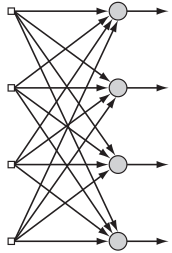
\includegraphics[width=0.25\textwidth]{imgs/feedforward-single}
     }
     \hfill
     \subfloat[\emph{Feedforward} com múltiplas camadas\label{subfig:multilayer}]{%
       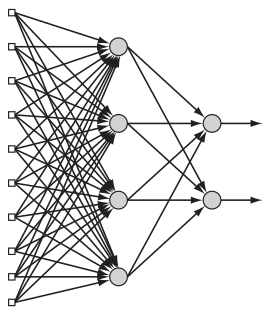
\includegraphics[width=0.35\textwidth]{imgs/feedforward-multi}
     }
     \hfill
     \subfloat[Recorrente\label{subfig:recurrent}]{%
       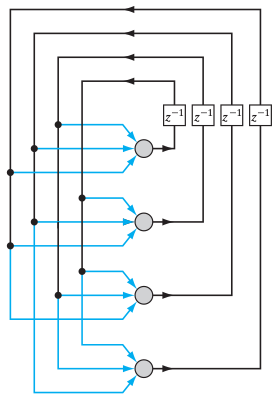
\includegraphics[width=0.3\textwidth]{imgs/recurrent}
     }
     \caption{Arquiteturas populares de RNAs. Fonte: \cite{haykin}}
     \label{fig:activation}
\end{figure}

Redes com múltiplas camadas, como na Figura \ref{subfig:multilayer}, caracterizam-se pela presença de pelo menos uma camada oculta. Segundo Cybenko, uma rede com uma camada oculta pode mapear qualquer função contínua, enquanto uma rede com duas camadas ocultas é suficiente para mapear qualquer função \cite{cybenko}.

\subsubsection{\emph{Multilayer Perceptron}}
\label{subsubsec:mlp}

As RNAs do tipo \emph{Multilayer Perceptron} (MLP), são redes constituídas do neurônio Perceptron, \emph{feedforward} e com múltiplas camadas, sendo estas uma camada de entrada, uma ou mais camadas ocultas e uma camada de saída. A arquitetura mais comum para uma rede MLP é a completamente conectada, de forma que os neurônios de uma camada estão conectados com todos os neurônios da próxima camada \cite{faceli}.

Em uma rede MLP, a função implementada por um neurônio de certa camada é uma combinação das funções realizadas pelos neurônios da camada anterior que estão conectados a ele. Na primeira camada, cada neurônio aprende uma função que define um hiperplano. Na camada seguinte, os neurônios combinam um grupo de hiperplanos, formando regiões convexas. Os neurônios da camada seguinte combinam então um subconjunto das regiões convexas em regiões de formato arbitrário \cite{faceli}. Na Figura \ref{fig:aprendizado-mlp}, tem-se uma visualização do processo ocorrido.


\begin{figure}[h!]
\centering
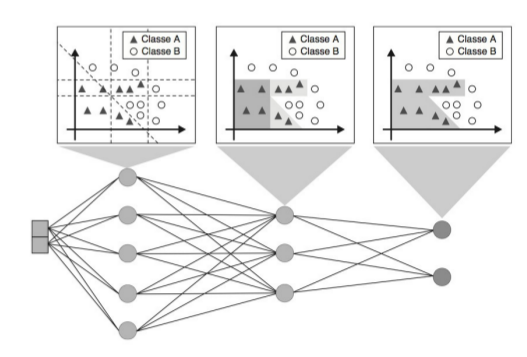
\includegraphics[height=6cm]{imgs/aprendizado-mlp}
\caption{Papel exercido pelos neurônios em cada camada de uma rede MLP. Fonte: \cite{faceli}.}
\label{fig:aprendizado-mlp}
\end{figure}

O algoritmo de aprendizado supervisionado mais conhecido e utilizado para treinamento das MLPs é o \emph{backpropagation}. Neste algoritmo utiliza-se as entradas e as saídas desejadas para o ajuste dos erros da rede. O treinamento ocorre em duas fases, a fase \emph{forward} e a fase \emph{backward}, em que cada fase percorre a rede em um sentido. Na fase \emph{forward}, a saída da rede é definida considerando certo padrão de entrada. A fase \emph{backward} utiliza a saída desejada e a saída fornecida pela rede para atualizar os pesos nas suas conexões \cite{braga}. O \emph{backpropagation} é simplesmente um método que utiliza o gradiente descendente para minimizar o erro quadrático total da saída calculada pela rede, na qual a derivada parcial define o ajuste dos pesos. Essa derivada mede a contribuição de cada peso no erro da rede para a classificação de dado objeto \cite{fausett, faceli}.

No âmbito do cálculo, o gradiente indica o sentido e a direção para os quais devem-se mover os valores dos pesos e dos bias nas camadas de forma a se obter o maior incremento possível de perda. Porém, nas técnica de \emph{backpropagation}, queremos mudanças de peso que trarão a inclinação mais íngreme ao longo da função de erro \cite{goodfellow, kubat}.

Um grande crescimento do poder computacional em termos de velocidade e memória tem acontecido nos últimos tempos. Dado isto, houve a viabilidade de treinamento das chamadas \emph{redes neurais profundas}, MLPs que possuem mais camadas escondidas do que o usual. Devido a ampla popularidade dessas redes e a capacidade computacional para a utilização de grande quantidade de dados de treinamento, foram desenvolvidas técnicas de \emph{deep learning} em pleno estado da arte para detecção, segmentação, classificação e reconhecimento de objetos em imagens \cite{khan}. Utilizando-se redes neurais convolucionais, podemos ainda elencar aplicações como o reconhecimento de padrões em imagens para uso na medicina \cite{cha}, a modelagem de frases por computadores \cite{kalchbrenner} e o reconhecimento de caracteres e dígitos \cite{lecun}. Essas e outras técnicas serão apresentadas mais profundamente nas seções a seguir.

% Backpropagation

%%%%%

\subsection{\emph{Deep Learning}}
\label{subsec:dl}

\subsubsection{Redes Neurais Convolucionais}
\label{subsubsec:cnns}

% Convolução
% Pooling
% Dropout
% Arquitetura canônica


\subsubsection{Arquiteturas canônicas de Redes Neurais Convolucionais}
\label{subsubsec:arq-cnns}

\subsubsection{\emph{Transfer Learning}}
\label{subsubsec:transfer}
